\chapter{Introduction}
There are vast amount of information and products available on the web. Even within a single websites the number of items can be overwhelming for users. Examples of sites where this applies are news sites, streaming services, and e-commerce sites. Recommender systems can help creating a better user experience by helping users find what they are looking for and are interested in. They can also help businesses in different ways, like showing targeted ads or help offering a better product.\\

In this paper, we will explore recommender systems, specifically session-based recommender systems. We will look at the use of deep learning and recurrent neural networks(RNN) for this, as compared to classical methods.\\

This introduction chapter introduces session-based recommender systems, some of the challenges in the domain, recurrent neural networks and how they fit into the problem.
The second chapter, State of the art, looks at different methods that exist, but focuses on what has been done in terms of deep learning and RNNs.
In the third chapter, Core, we explain our own work.
Our experiments and results are laid out in the fourth chapter, Experiments and results.
Lastly follows a the conclusion and further work, which summarize what has been done, which challenges remain and needs to be studied further.

%----------------------------
%Give short introduction about what this report will discuss (rnn), touch very briefly upon what the reader should have in mind and can expect from the report. Explain what will be discussed in the different chapters.
%
%Touch very briefly upon what rnn is, so that the reader understands enough to understand the next sections, before we get to background. (Or should background come before motivation and objectives of work?)


\section{Motivation}
\label{sec:motivation}

As mentioned, recommender systems can help both users looking for content and the providers of the content. Users are generally interested in finding what they are looking for as easy as possible, or to be shown products or content that interests them, but which they normally would not have discovered on their own. Spotify helps users discover new content introducing them to new music, tailored to the user, through their Discover Weekly\cite{discover-weekly} playlists. When a user buys something on an e-commerce site like Amazon, the site display items to the user, that other users bought together with the original item. These are examples where recommender systems helps users discover new content and helps user find products they are interested in.\\

For the provider, or seller, there may be different reasons to use recommender systems depending on their business model. Google earn money when users click on ads, so it is important for them to show relevant ads with high probability of getting clicked by the user. Similarly, YouTube earns money by showing commercials in their videos, and thus they can earn more money by making the user watch more videos. This can be accomplished by suggesting videos that the user wants to watch. Or like in the Amazon example, suggesting additional items might make the buyer but more than he had initially intended. Recommender systems are also used by Facebook and news feeds which tries to filter out what is shown to the user.\\

%Why are recommender systems interesting? (interesting for both users and provider/seller) occour in many situations, especially on the web, ads placement on sites like google and finn.no, music on spotify, movies on netflix, media content on youtube, any webshop what so ever, facebook...

In the examples above, recommendations are made based on the user profile, which has information about the user interests. This profile is built up over time, as the user interacts with a system/site. Or in the Amazon example, the recommendation may only be based on a single or few items that the user bought. To make good recommendations in these scenarios, it is assumed that one has access to a user profile, but this might not always be the case. Multiple users may share an account, maybe the user is new, or maybe the user is not logged in at all. Sites can use cookies to get some historical data about the user when he is not logged in, but this is not very reliable either. There might not exist any cookies because the user is completely new to the site, or he may have deleted them. And even though we have access to cookies with information, the traffic might come from a computer shared by family members for example. Son and mom are probably not buying the same clothes, or listening to the same music. But even when we assume that it is possible to know who the user is, and what his interests are, he might be searching for content/products that is not related to his interests at all. An example of this could be a professional angler that wants to buy beginner equipment for his nephew, or maybe the angler suddenly has decided to start playing football and is looking for football equipment. Another example is a programmer who wants to listen to calm classical music while he works, but when he goes to the gym after work, he wants to listen to energetic techno. In these situations the recommender system will not be able to make good recommendations based on what it knows about the user. Only the current session might be relevant to what the user is looking for.\\

%Why are they interesting in the session-based setting? (don't have user profile, don't know what the user likes, still want to give good recommendations. Would be nice if we could do better than just recommending generally popular or similar items)
%Maybe different users use the same account (netflix), or the traffic comes from a family computer where different family members have very different interests.
%Even a single user may have vastly different interest from time to time. A user may look for different things depending on holidays or events, and he might be looking for different things during and after work hours. Also, especially in the case of shopping, a user might be looking for items not related to his interest at all, so the only info we have for recommendation is the current session. 

Recurrent neural networks intuitively fits well as a recommender system, especially in the session-based scenario. They do not suffer from the cold start scenario, they can perform well with minimal information about items, and they make it easier to extract good features \cite{ZALANDO:understanding-consumer-histories}. Also, RNNs does not suffer from some of the assumptions that classical neural networks do. With recent advances in architectures for RNN, ways to circumvent training problems, and better hardware, RNNs have become very feasible to use. Much research has been done on RNNs recently, some of this research focuses on using RNN as a session-based recommender system. The results are promising, and it seems like RNNs are fully capable of competing with state of the art recommender systems.

%Why are RNN interesting? with invention of the LSTM and GRU units, combined with better hardware, they have become much more feasible to use

%RNNs have properties that intuitively fits in a recommender system, and maybe moreso in the session-based variant.

%RNN does not suffer from the cold start scenario, makes it easier to extract good features, and can even perform well with no information about items.


%---------------------------
%Why are RNNs interesting?
%- easier feature extraction/engineering (zalando blog)
%- the model fits very well with problems involving sequences. can model sequences, has memory
%- has achieved very promising and state of the are results 
%- has recently become interesting because of lstm, gru which helps with vanishing and exploding gradients, pluss powerful hardware
%- does not suffer from cold-start problem. can apply on unknown users
%- can easily work with sequences of different length

\section{Objectives}
The goal of this paper and the work described in it, is to implement an RNN and test how it performs as a recommender system. We explore recommender systems, particularly those that deal with session-based recommendation. Specifically we look at the use of RNNs as session-based recommender systems. We want to know if they can compete with other models currently in use. Furthermore, we look at different architectures and ways of optimizing them to improve results. Our work is inspired, mainly, by the work in \cite{DBLP:journals/corr/HidasiKBT15} and \cite{DBLP:journals/corr/LiuWWL016}. The first paper explores the use of an RNN for session-based recommendations compared to other methods. The second paper explores how adding context information as input to the network can improve the results.


%implement an rnn and test its performance as a recommender system.
%explore recommender systems, specifically session based. Explore the use of using rnn for this instead of classical methods. The work is inspired by paper x, y, z, and these are used as a basis for our exploration. 

%-----------------------

%- look at work that has been done, state of the art
%- look at how results can be improved when predicting sequences
%- specifically interested in situations that apply to online users where we might have no prior knowledge of the user

\section{Background}
In this section we explain, on a high level, terms and concepts used in this paper.

\subsection{Recommender systems}
As touched upon in \ref{sec:motivation}, recommender systems are systems that try to predict a users evaluation of an item, or what items a user is interested in interacting with. They can be, and are, used in many areas. Some examples are music, movies, news, restaurants, recipes, online shopping, and dating. Figure \ref{fig:recsys-example-xbox} shows an example of recommendations made by Amazon and YouTube when looking at a Xbox One.\\
	
\begin{figure}[htp]
	\centering
	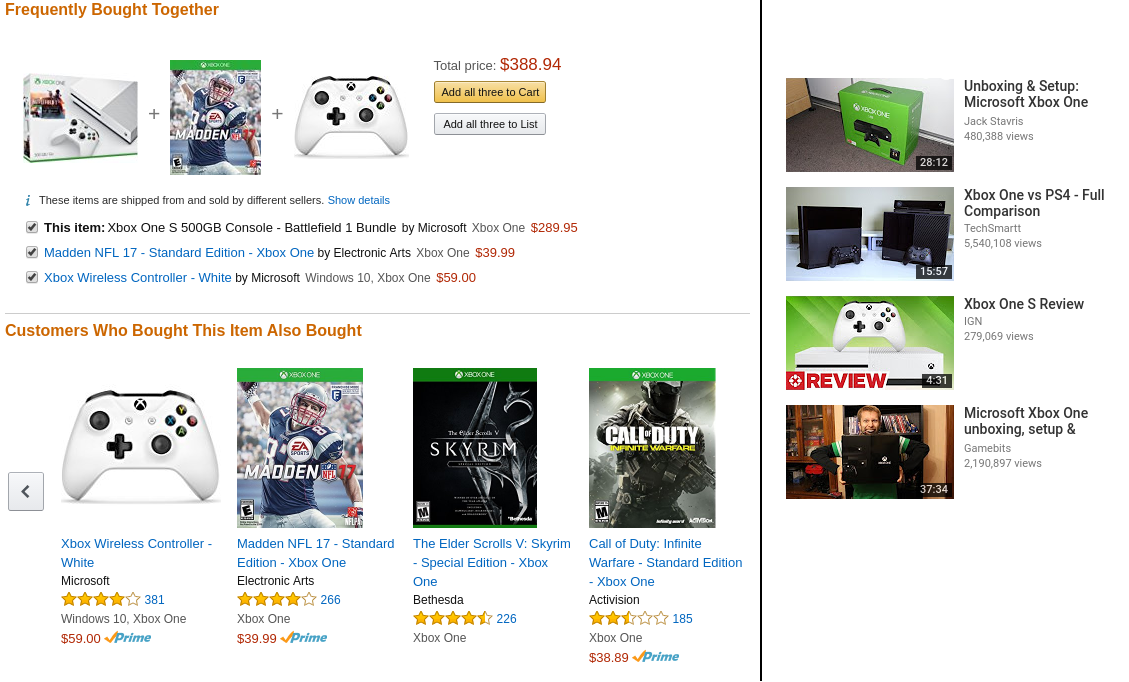
\includegraphics[width=1.1\textwidth]{fig/recsys_example_xbox.png}
	\caption{Recommendations from Amazon (left) and YouTube (right) when looking at Xbox One.}
	\label{fig:recsys-example-xbox}
\end{figure}

Note that there is a subtle difference between predicting which items a user will like, and which items he is interested in interacting with. The former case involves predicting what rating a user will give a movie or whether a user is likely to purchase one or any item. On the other hand, the latter case does not worry about how the user will interact with an item, but whether the user will choose to interact with the item, given the choice. To exemplify this, lets look at a movie streaming site. Should the site recommend movies that the user will rate highly if he watches them, or should it recommend movies that the user is likely to watch independent of how he will rate it? The answer will probably depend on the business and other factors, the point is that there is a difference between the two approaches. In the movie example, it is reasonable to think that how a user would rate a movie is less dynamic than what he want to watch. His ratings would probably depend a lot on his personal preferences, which usually change slowly over time. What he is interested in watching at any point, however, might depend more on circumstances. This was illustrated earlier with the worker who wanted to listen to different genres at during work and his workout session.\\

It is therefore clear that the goal of recommender systems may vary with different businesses and settings. In this paper we are mainly concerned with predicting the next item the user will choose to interact with.\\

There are two classical approaches to recommender systems, collaborative filtering and content-based filtering. These two methods can be combined into a hybrid approach.

\subsection{Collaborative filtering}
Collaborative filtering uses information about users preferences to recommend items highly rated by similar users. To illustrate, let us look at a movie recommendation system. A user logs into a website where he can rate movies he has seen, and the site recommend movies to the user, based on his ratings. With the collaborative filtering approach, the user needs to rate some movies to get good recommendations, and as the user rate more and more movies, the system is able to make better recommendations. To make the recommendations, the system groups together similar users. A user is then recommended movies that he has not seen and that was rated highly by other similar users. The system decides whether users are similar by looking at how like-minded they are, that is, how similar they rate movies. This is illustrated in figure \ref{fig:collaborative-filtering}. The system predicts what rating the question mark will be by guessing the same rating as those given by similar users (highlighted in green).\\

\begin{figure}[htp]
	\centering
	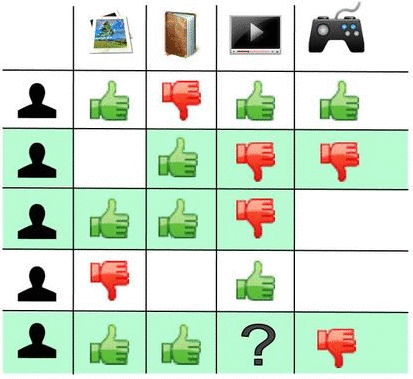
\includegraphics[width=0.4\textwidth]{fig/collab-filtering.png}
	\caption{Illustration of collaborative filtering}
	\source{https://en.wikipedia.org/wiki/Collaborative\_filtering\#/media/File:Collaborative\_filtering.gif}
	\label{fig:collaborative-filtering}
\end{figure}

Many sites have a huge amount of items, and the average user only interacts with a handful of these, this creates a sparsity problem for collaborative filtering methods. These methods also face the cold start problem.\\

One of the most popular collaborative filtering algorithms is matrix factorization \cite{matrix-factorization}.

\subsection{Cold start}
The cold start problem occurs when a recommendation approach is based on having a large amount of data on the user. When a new user occurs the model is not capable of making accurate recommendations due to the lack of user information. Collaborative filtering methods suffers from the cold start problem, but when they do have access to rich user information, they are usually able to make better recommendations than content-based filtering methods.\\

Due to the cold start problem, collaborative filtering approaches alone, are not well suited for session-based recommendations.

\subsection{Content-based filtering}
Content-based approaches builds a user profile based on the item interactions of the user, and features of items. For example, if a user watches a lot of western movies or movies with a certain actor, the system can infer that the user likes the western genre or is a fan of that actor. Then, the system can recommend movies within the western genre or movies where the actor appears. So the approach is to build a user profile based on the profile of the items he interacts with.\\

To achieve good results with content-based filtering, it is important to create accurate item profiles with representative features. The content-based approach does not suffer from the cold start problem to the same degree as collaborative methods, but content-based methods are more limited in their recommendations. They are only able to recommend items similar to those the user has already interacted with. With respect to this, the collaborative filtering approach might offer more valuable recommendations.\\

Some content-based approaches include decision trees, neural networks, and cluster analysis.


\subsection{Session-based recommender systems}
Session-based recommender systems tries to do predictions mostly based on the current user session. Sessions are often limited in time, and, as we have seen, the users interests might vary between sessions. Generally we no information about the user, and since the sessions are short, we do not get much information either. There may be many reasons for this lack of information. Some examples are new users, users sharing accounts, and small e-commerce sites where each unique user only visits it a couple of times. Furthermore, even though we have access to information about the users interest, this might be of minimal use if the users interests vary greatly between sessions. A session usually consists of multiple user actions on a number of items, in the order the actions happen, constrained to a short timespan. What ''short timespan'' means will depend on the domain, but it is often in the order of minutes or a few hours.\\

\subsection{Neural networks}
Neural networks are models inspired by the human brain. They consist of layers of neurons, often referred to as nodes or units, who can receive an input signals, and depending on the strength of the signals, output signals of its own. The nodes are grouped together in layers, and the nodes in each layer output values to the next layer based on the input from the last layer. Values can also be sent back into the same layer they originated from. Each neuron can receive values from multiple neurons, and each neuron can output values to multiple neurons. Each input value to a neuron is weighted, and all the weighted inputs are summed together. A bias might also be added to this sum. This sum is sent through a function, called the activation function, and the function value is passed on to the next neurons. This is illustrated in figure \ref{fig:neural-network}. Mathematically, the layers can be represented as vectors, where each index corresponds to one node, the weights can be stored in a matrix and matrix multiplication can then be used to successively compute the vector for each layer.\\

\begin{figure}[htp]
	\centering
	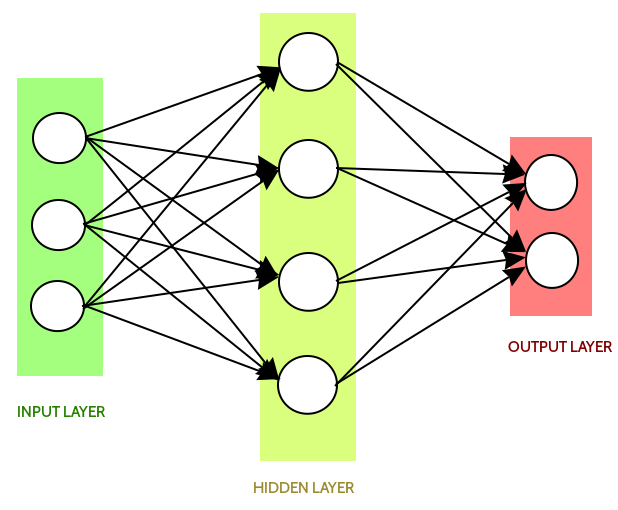
\includegraphics[width=0.8\textwidth]{fig/neural-network.png}
	\caption{A feed forward network. Exmaples are inserted into the network by setting the values in the input layer. The values of the nodes in each layer are computed as a function of the values in the nodes in the prior layer.}
	\label{fig:neural-network}
\end{figure}

An example application might be to let a neural network guess whether it is going to rain in the afternoon, by presenting it with values representing different conditions in the morning. These conditions, or features, could be temperature, air humidity, and whether it rained yesterday. To feed the network these features, they need to be encoded into a vector of real values. This could be done by using a vector with 5 dimensions, where the first index is a 1 or 0, indicating whether it rained or not yesterday. The second index could be the air humidity, scaled down to the range (0,1). And finally, the last 3 indexes could be used to represent the temperature, for example, by creating three buckets. If the temperature is above 20 \degree C, the third index would be set to 1, the fourth if the temperature is between 0 \degree C and 20 \degree C, and the fifth index would be used if the temperature is below 0 \degree C. The output layer could be a vector with 2 dimensions, where one index would indicate rain, and the other would indicate no rain. Then the index with the highest value could be used as the networks prediction.\\

The layers between the input and the output layers are called hidden layers. A neural network can any number of hidden layers, this includes not having a hidden layer at all. The width of a layer is the number of nodes in the layer. Adding more layers to a network increases its capacity, which means that it becomes capable of solving more complex problems. However, with more layers, the network also becomes harder to train, both in terms of number of calculations and because more layers creates a bigger, and more complex search space.\\

The most popular ways of training uses backpropagation. Different variations exists, but the main idea is the following. First the network is presented with an example, and the values of all the nodes in the network is computed. Error values are calculated for the output layer, based on its difference from the target output. These errors are then backpropagated through the network. This means that the error in each node is dependent on the input it gets from the previous, upstream, nodes. So the error of the upstream nodes can be calculated by how much they contributed to the error in the downstream nodes. Based on this, the weights in the network can be adjusted. Let us look at a very basic example. A single output node, \textit{O}, ends up with the value 1. This is the sum of 2 and -1, which \textit{O} got from nodes \textit{A} and \textit{B} respectively. If the target value of \textit{O} was 0.5, then the weights from \textit{A} and \textit{B} to \textit{O}, should be adjusted so that the sum of the inputs gets skewed towards 0.5. So after the adjustments, \textit{A} and \textit{B} would output 1.75 and -1.25 instead, on the same example. Exactly how the weights are updated, depends on the chosen training algorithm and the parameters used, but the main idea is mostly the same.\\

In more correct terms, the output error is calculated with a loss function. Greater error means greater loss. But the loss does not have to be as simple as the difference between the target values and the computed values, more delicate functions can be applied. The most successful algorithm for training neural networks is called backpropagation and was introduced by Rumelhart et al. in 1985 \cite{DBLP:journals/corr/Lipton15} \cite{Rumelhart:1986:LIR:104279.104293}. Backpropagation uses the chain rule to calculate the derivative of the loss function L with respect to each parameter in the network. The weights are then adjusted by gradient descent \cite{DBLP:journals/corr/Lipton15}.

Figure \ref{fig:neural-network} shows a fully connected feed forward network. Fully connected means that each node in a layer is connected to all the nodes in the next layer. Feed forward means that there are no cycles or recurrent connections, all connections go to the next layer, towards the output layer.

\subsection{Dropout}
Dropout is a regularization technique that can be used when training neural networks. As the name implies, a subset of the nodes are deactivated. Deactivating subsets of the nodes during training, can help avoid overfitting and it can speed up the training \cite{Srivastava:2014:DSW:2627435.2670313}. Speed up is achieved because there are less nodes to train. By randomly deactivating node, the network becomes more robust, since it cannot rely to much on any one node to produce good results.

\subsection{Minibatches}
When training neural networks, one can calculate the error for multiple training examples and then update the weights based on the average of these examples. These groups of examples are called minibatches. There are several benefits of using this. Using large batches generally results in a more accurate estimate of the actual error of the model. For example if some of the examples are outliers. With a better estimate of the real error, the training algorithm can use a higher learning rate. Also, some hardware can be better utilized when training with batches. \cite{Goodfellow-et-al-2016-Book}

\subsection{Deep learning}
The small network shown in figure \ref{fig:neural-network} is not capable of learning very complex tasks, it is too simple.  Increasing the size of the layers would probably give it some more capacity. If we wanted to do image labeling, the task of recognizing objects in an image, with it we could increase the input layer so that it had three nodes for each pixel (RGB). We would also have to increase the output layer to have one node for each possible label. However, even with a huge hidden layer, the model will struggle to make sense of raw pixels with only a few calculations. To help the model, we could give it additional input, we could tell it whether geometric figures like circles exists in the image. But by doing this, we have started to do some of the image labeling ourselves. Also, the model is dependent on us being able to find good features for it. We want the model to do most of the work for us. It would be nice if the model could extract good features by itself. It turns out that it can.\\

By adding more hidden layers to our model it becomes much more capable. In its simplest explanation deep learning is just that, using more layers. This does not just apply to neural networks, one can also stack layers of other artificial intelligence methods, but we will focus on neural networks. The great benefit of using deep models is that the models are able to learn and extract good features themselves \cite{Goodfellow-et-al-2016-Book}. In the case of image labeling, the first layers can learn to extract features like edges and simple shapes. The deeper layers can then use these features to recognize more complex shapes in the image. Or in the case of recommender systems, the model can learn to extract features from the items and user preferences from user actions. Deep learning lets the machine learn hierarchical concepts, giving it more power and flexibility \cite{Goodfellow-et-al-2016-Book}.

\subsection{Recurrent neural networks}
Recurrent neural networks(RNN) area form of neural network that is suited for processing sequences of data. Standard neural networks have no form of memory between examples, they assume that each example is independent, which often is not true. RNN solve this by using loops where information from the one time step is passed on to the next one. This gives the model memory, and it does not need to assume independence between examples. It also means that the model is more suited for sequences of varying lengths. Figure \ref{fig:rnn} illustrates a basic RNN. It can be illustrated both as a loop and as an unrolled network. Note that, as implied by the looped representation, the RNN is the same across all time steps. In the unrolled version, the RNN boxes are the same network, there are not \textit{t} different RNNs that are connected.\\

\begin{figure}[htp]
	\centering
	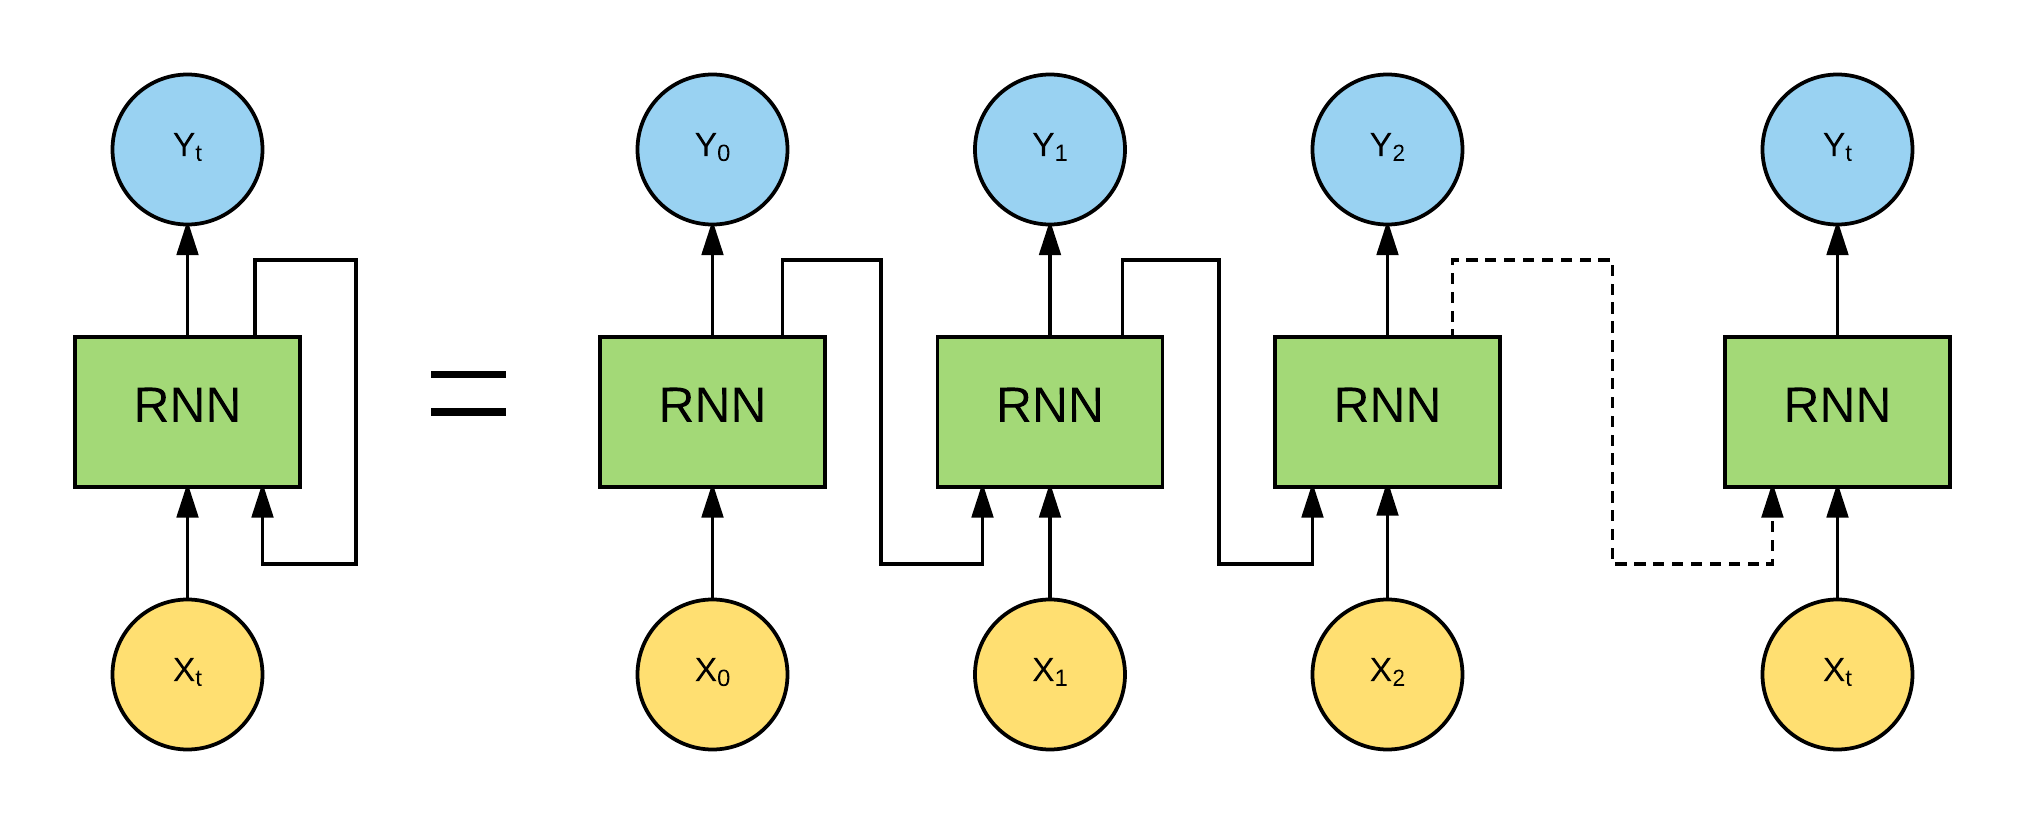
\includegraphics[width=1.0\textwidth]{fig/rnn.png}
	\caption{A simple RNN. Represented as a loop(left), and unrolled to \textit{t} timesteps(right).}
	\label{fig:rnn}
\end{figure}

At each time step, the network takes in external input and input from the last time step, two outputs are created. One output is passed on to the output layer, or the next hidden layer if there is one. The other output is the state of the RNN, which is passed on to the next time step. Each time step does not have to be separated by a fixed amount of time, each time step is just when input arrives. It is fully possible to apply deep learning to RNNs. One can stack multiple RNNs, or add other types of layers such as a plain feed forward layer.\\

RNNs are not constrained to neither fixed sized inputs nor outputs. The size of input and output \textit{vectors} are fixed, but RNNs are not limited to a fixed number of such vectors. However, RNNs can be applied both to domains where it is natural to treat the data as sequences, as well as problems where the amount of input is fixed. An example of this is to use a RNN as a sliding window over fixed sized images.


\subsection{LSTM and GRU}
Early RNN had troubles with training because of vanishing and exploding gradients. When using many time steps the gradients often grew too steep, exploded, or they approached zero, vanished. This problem happened because the recurrent edge in a node always had the same weight, which resulted in the derivative of the error either exploding or approaching zero, at an exponential rate, as the number of time steps grew \cite{DBLP:journals/corr/Lipton15}. This was solved by introducing a memory cell. The new model introduced by Hochreiter and Schmidhuber in 1997 and is called \textit{long short-term memory}(LSTM) \cite{Hochreiter96bridginglong}. Improvements to the original model has been made over time. In the LSTM model, each node in the recurrent layer is replaced by a memory cell. The internal structure of the memory cell is a bit complex, but simply explained it has an internal state that it can modify, in addition to the old features of RNN nodes. So, the cells can decide how much information in the internal state they want to keep at each time step, and how much new information they want to add.\\

GRU

\subsection{RNN as a session-based recommender system}
Explain how RNNs fit into the session-based context

%theoretical background. explain everything at a high level (more technical explanations can be done in state of the art). Everything that is used in the core

%- What is a recommender system?
%   Why do recommender systems exist
%   Two sligthly different types of recommender systems (predict what the user will give a good rating, and predict what the user would want to interact with independently of whether he will give it a good rating or not)
%- What is a session-based recommender system?
%- What is a neural network
%- What is deep learning
%- What is RNN
%- GRU and LSTM
%- Contextualise what I am doing
%- what is contextual information (external [time, weather, ...] and item specific context [more info abiout the item: image, text, category...])

%-----------------------
%- explain the problem domain
%- explain rnn